%% Based on a TeXnicCenter-Template by Gyorgy SZEIDL.
%%%%%%%%%%%%%%%%%%%%%%%%%%%%%%%%%%%%%%%%%%%%%%%%%%%%%%%%%%%%%

%------------------------------------------------------------
%
\documentclass[a4paper,12pt]{article}%
%Options -- Point size:  10pt (default), 11pt, 12pt
%        -- Paper size:  letterpaper (default), a4paper, a5paper, b5paper
%                        legalpaper, executivepaper
%        -- Orientation  (portrait is the default)
%                        landscape
%        -- Print size:  oneside (default), twoside
%        -- Quality      final(default), draft
%        -- Title page   notitlepage, titlepage(default)
%        -- Columns      onecolumn(default), twocolumn
%        -- Equation numbering (equation numbers on the right is the default)
%                        leqno
%        -- Displayed equations (centered is the default)
%                        fleqn (equations start at the same distance from the right side)
%        -- Open bibliography style (closed is the default)
%                        openbib
% For instance the command
%           \documentclass[a4paper,12pt,leqno]{article}
% ensures that the paper size is a4, the fonts are typeset at the size 12p
% and the equation numbers are on the left side
%
\usepackage{amsmath}%
\usepackage{amsfonts}%
\usepackage{amssymb}%
\usepackage{graphicx}
\usepackage{geometry}
\usepackage[hidelinks]{hyperref}
\usepackage{svg}
\usepackage{tabularx}
\usepackage{array}
%-------------------------------------------

\newcolumntype{C}{>{\centering\arraybackslash}X}
\geometry{margin=1in}
\setcounter{secnumdepth}{5}
\setcounter{tocdepth}{5}
\newcounter{assumptions_counter}
\newcounter{goals_counter}
\newcounter{func_req_counter}
\newcommand{\usecasetable}[5]{
\begin{center}
\begin{tabularx}{\textwidth}{|X|C|}
\hline
Actor & #1\\
\hline
Goal & #2\\
\hline
Event Flow & #3\\
\hline
Output Condition & #4\\
\hline
Exception & #5\\
\hline
\end{tabularx}
\end{center}
}
\newcommand{\defsw}[4] {
\begin{itemize}
\item #1:
\begin{itemize}
\item Name: #2
\item Version: #3
\item Source: #4
\end{itemize}
\end{itemize}
}
\begin{document}
\begin{figure}
  \centering
	\def\svgwidth{\columnwidth}
    \resizebox{0.35\textwidth}{!}{\input{logo_polimi.pdf_tex}}
\end{figure}
\title{{\Huge \textbf{R}equirements \textbf{A}nalysis and\\
\textbf{S}pecification \textbf{D}ocument}\\{\Large Software Engineering 2: ``myTaxiService''}}

\author{Fioratto Raffaele, Longoni Nicol\`{o}
\\Politecnico di Milano
\\{\small A.Y. 2015/2016}}
\date{October 22, 2015}
\maketitle
\newpage
\tableofcontents
\newpage
\section{Introduction}

\subsection{Purpose}
This document represents the Requirement Analysis and Specification Document
(RASD). The main goal of this document is to describe completely the system
in terms of functional and non-functional requirements, analyzing real needs
of customers to model the system, showing constraints and limits
of the software and simulating typical use cases that will occur after the
development. This document is addressed to all developers and programmers who
have to implement the requirements, to system analysts who want to integrate
other systems with this one, and could be used as a contractual basis between
the customer and the developer.

\subsection{Actual System}
The software house wants to offer a new service to optimize an existing 
taxi service of a large city. We suppose that until now, nothing has been 
created and we have to create the entire application without using or modifying 
a previous system.

\subsection{Scope}
The aim of the project is to create a new brand system that optimizes an 
existing taxi service.
The system will be capable of automatizing  and/or simplifying certain 
processes during requests or reservations of taxis.
It will also guarantee a fair management of taxi queues.
New passengers can sign up for service inserting some basic information in order to use service's features as soon as possible.
A passenger can request a taxi using web service or through mobile
application after registration. The system will be able to localize precisely the position
of the passenger, determining the taxis that are available near
him/her. The system will select a taxi and then will forward the request to its driver.
Upon confirmation, the system will notify the customer about the successful completion of the operation and the ETA of the taxi. A passenger can also reserve a taxi by specifying the time and the date.
Passengers who want to reserve a taxi should do it with at least two hours in advance, cancellation is also permitted. The system will actually process the request ten minutes before the time specified during the reservation in the same way as described previously.

\subsection{Actors}
\begin{itemize}
\item Unregistered Passenger: a person that is not registered to the system, i.e. a visitor. He/she can only visit the registration page.
\item Registered Passenger: all customers that have a valid username and password and that are able to access all available features to customers, they can request or reserve a taxi, they can also cancel these operations with some constraints later explained.
\item Taxi Driver: a person who is able to drive a taxi, owns a valid 
professional driving license. The driver informs the system about the availability of his/her taxi, logging in a specific mobile application installed in his/her smartphone, and do the same when the ride ends. 
\item System Administrator: the person in charge of updating the list of the actual cars and the list of qualified drivers.
\end{itemize}
\subsection{Goals}
List of goals for myTaxiService system:
\begin{itemize}
\stepcounter{goals_counter}
\item \nameref{goal\arabic{goals_counter}}
\stepcounter{goals_counter}
\item \nameref{goal\arabic{goals_counter}}
\stepcounter{goals_counter}
\item \nameref{goal\arabic{goals_counter}}
\stepcounter{goals_counter}
\item \nameref{goal\arabic{goals_counter}}
\stepcounter{goals_counter}
\item \nameref{goal\arabic{goals_counter}}
\stepcounter{goals_counter}
\item \nameref{goal\arabic{goals_counter}}
\stepcounter{goals_counter}
\item \nameref{goal\arabic{goals_counter}}
\stepcounter{goals_counter}
\item \nameref{goal\arabic{goals_counter}} 
\stepcounter{goals_counter}
\item \nameref{goal\arabic{goals_counter}} 
\end{itemize}
\subsection{Definitions, Acronyms, Abbreviations}
\subsubsection{Definitions}
\begin{itemize}
\item 
\end{itemize}
\subsubsection{Acronyms}
\begin{itemize}
\item RASD: Requirements Analysis and Specification Document
\item DB: DataBase
\item DBMS: DataBase Management System
\item API: Application Programming Interface
\item ETA: Estimated Time of Arrival
\item OS: Operating System
\item FIFO: First-In First-Out
\item JVM: Java Virtual Machine
\item RPC: Remote Procedure Calls
\item JSON: JavaScript Object Notation
\end{itemize}
\subsubsection{Abbreviations}
\begin{itemize}
\item {[}Gn{]}: n-goal %curly braces needed to escape '[' and ']'
\item {[}Rn{]}: n-functional requirement
\item {[}Dn{]}: n-domain assumption
\item {[}Fn{]}: n-figure
\item {[}An{]}: n-assumption
\end{itemize}
\subsection{Identify Stakeholders}
Our main stakeholders are government members of the city that are interested in optimizing the existing taxi service.
Other stakeholders can be companies that want to enhance the service as well, but also the passengers and taxi drivers who want a more comfortable, intuitive and user-friendly service.
\subsection{Reference Documents}
\begin{itemize}
\item myTaxiService Specification Document
\item IEEE Std 830-1998 IEEE Recommended Practice for Software 
Requirements Specifications.
\end{itemize}
\subsection{Document overview}
The document is essentially divided into four parts:
\begin{itemize}
\item Section 1: Introduction, it gives a description of this document and some basic information about software utilized.
\item Section 2: Overall Description, gives general information about the software to project, focused on constraints and assumptions.
\item Section 3: Specific Requirements, this part lists requirements, typical scenarios and use cases. To give an easy way to understand all functionality
of this software. This section is filled with UML diagrams.
\item  Section 4: Appendix, this part contains some information about the attached files and some described screenshots of software used to generate
it.
\end{itemize}
\newpage
\section{Overall Description}
\subsection{Product perspective}
The final product will consist of a web service and a mobile application for customers and taxi drivers.
The overall system will also have an internal interface for the system administrator. The system should also interact with existing external services, and will also provide additional APIs that allows the development of additional features in the future. 
\subsection{User characteristics}
The final customer that wants to use this application is a person who wants to move around the city using taxis in a easier and faster way than an ordinary taxi service can assure. This user must have some kind of digital equipment that let him access the Web by means of a modern browser. The user can also use the mobile application to have a more enhanced user experience using this service.
From the system administrator perspective, he expects a very intuitive interface that enables a fast way to manage the back-end information. We expect that an already hired employee will be trained to do such job.
\subsection{Constraints}
\subsubsection{Regulatory policies}
For the myTaxiService we have identified the following regulatory policies:
\begin{itemize}
\item Cookies: since it is mandatory to log in the web service to interact with the system, it is necessary to use cookies in order to keep track of each user's session, thus the system must comply with the current Cookie Law.
\item Privacy: the system needs to manage some sensible data of customers and taxi drivers, for instance the name, the surname, an e-mail etc. Another crucial information is the current location detected by GPS of both. During the registration, customers must accept the Privacy Law (see login mockup), regarding taxi drivers, before being registered to the system by the administrator, drivers have to sign a document, accepting the processing of its personal data.
\item Drivers during their work are subject to the Traffic code.
\item The workday of a driver is subjected to the laws about Job safety, so the system must allow the driver to take some breaks during the day in order to prevent both illnesses, damage to people, tiredness problems and stress.
\end{itemize}
\subsubsection{Hardware policies}
For the myTaxiService we have identified the following regulatory policies:
\begin{itemize}
\item Smartphone: because of their limited power and battery, we must take care of application consumption and also web services (for instance, implementing a responsive design).
\end{itemize}
\subsubsection{Interfaces to other applications}
\begin{itemize}
\item Google Maps: it will be used to provide passengers an estimation of taxis arrival time.
\item External Database: it contains information about the drivers' license and data about cabs, the system will interrogate this database to check the correctness of the information supplied by taxi drivers during the registration in the system.
\end{itemize} 
\subsubsection{Parallel operation}
myTaxiService must support parallel operations from different users when it works
with database and with all operations done by users after connections.
\subsubsection{Documents related}
\subsection{Assumptions and Dependencies}
\subsubsection{Assumptions}
\begin{itemize}
\stepcounter{assumptions_counter}
\item \label{a\arabic{assumptions_counter}}{[}A\arabic{assumptions_counter}{]}
Only registered users can use the service, because additional information such as name, surname and e-mail to confirm and to recap the reservation are needed, to avoid repetition, the user has to re-enter this information every time.
Another reason is to prevent passengers to make requests to the system while another one is in processing.
\stepcounter{assumptions_counter}
\item \label{a\arabic{assumptions_counter}}{[}A\arabic{assumptions_counter}{]} Passenger position is exactly known thanks to the usage of GPS available in smartphones or by using a geolocalization API from browser. 
\stepcounter{assumptions_counter}
\item \label{a\arabic{assumptions_counter}}{[}A\arabic{assumptions_counter}{]} The position of the taxi is exactly known by using the GPS available in the driver's smartphones
\stepcounter{assumptions_counter}
\item \label{a\arabic{assumptions_counter}}{[}A\arabic{assumptions_counter}{]} The city is divided into zones of 2 $km^2$ each and for each zone a taxi queue is allocated.
\stepcounter{assumptions_counter}
\item \label{a\arabic{assumptions_counter}}{[}A\arabic{assumptions_counter}{]} The driver can take at most 2 breaks during his/her workday, during breaks the taxi belonging to him/her is not available.
\stepcounter{assumptions_counter}
\item \label{a\arabic{assumptions_counter}}{[}A\arabic{assumptions_counter}{]} A taxi driver must own a valid professional driving license and a cab with all documents in order
\stepcounter{assumptions_counter}
\item \label{a\arabic{assumptions_counter}}{[}A\arabic{assumptions_counter}{]} Each taxi driver's license has a unique code that identifies it
\stepcounter{assumptions_counter}
\item \label{a\arabic{assumptions_counter}}{[}A\arabic{assumptions_counter}{]} Each taxi cab has a unique code that identifies it
\stepcounter{assumptions_counter}
\item \label{a\arabic{assumptions_counter}}{[}A\arabic{assumptions_counter}{]} An external database with all the correct and up to date information about the taxi drivers and their cars (valid driving license, cars allowed to circulate in streets, etc.)
\stepcounter{assumptions_counter}
\item \label{a\arabic{assumptions_counter}}{[}A\arabic{assumptions_counter}{]} The existing taxi service is available 24 hours per day, 365 days per year.
\end{itemize}
\subsection{Future possible implementation}
\begin{itemize}
\item Allow customers to pay using an electronic payment system. During registration the passenger will provide additional information about his/her credit card or PayPal e-mail, the system will charge a ride automatically.
\item Extend the interface usable by customers to provide the ability to evaluate the service in general as a feedback to improve the overall system.
\item Expand the system to allow the possibility to share a taxi with other customers using the existing API.
\end{itemize}
\newpage
\section{Specific Requirements}
\subsection{External Interface Requirements}
\subsubsection{User Interfaces}
\subsubsection{API Interfaces}
The application on the server side will provide some APIs that are used by the mobile application to interact with the system itself. These APIs are essentially RPCs with the data encapsulated using JSON exposed using some endpoints (i.e. specific URLs). The mobile application will connect to the central application by means of this endpoints and will perform the necessary operations.
\subsubsection{Hardware Interfaces}
The system doesn't support any Hardware Interfaces.
\subsubsection{Software Interfaces}
\defsw{DBMS}{MariaDB}{10.0}{https://mariadb.org/}
\defsw{JVM}{Oracle JEE}{8}{http://www.oracle.com/technetwork/java/javaee/overview/index.html}
\defsw{Application Server}{Glassfish}{4.1.1}{https://glassfish.java.net/}
\defsw{OS}{Any operating system that can run host a DBMS application and the JVM}{N/A}{N/A}
\defsw{Mobile OSes}{Android}{$\geq$ 4.0}{https://www.android.com/}
\defsw{Mobile OSes}{iOS}{$\geq$ 7.0}{http://www.apple.com/ios/}
\defsw{Mobile OSes}{Windows Phone}{$\geq$ 8.0}{https://www.microsoft.com/en-us/windows/phones}
\subsubsection{Communication Interfaces}
\begin{center}
\begin{tabular}{|c|c|c|}
\hline
Protocol & Application & Port \\
\hline \hline
TCP & HTTPS & 443 \\
\hline
TCP & HTTP & 80 \\
\hline
TCP & DBMS & 3306 (default) \\
\hline
\end{tabular}
\end{center}
\subsubsection{Memory}
The minimum memory requirements are:
\begin{itemize}
\item Primary memory: 2GB+
\item Secondary memory: 20GB+
\end{itemize}
For the mobile application at least 512MB of primary memory is required in order to have a satisfactory user experience.
\subsection{Functional Requirements}
\setcounter{goals_counter}{1}
\stepcounter{func_req_counter}
\subsubsection{\label{goal\arabic{goals_counter}}{[}G\arabic{goals_counter}{]} Allow unregistered passengers to sign up for the service}
\stepcounter{goals_counter}
\begin{itemize}
\item {[}R\arabic{func_req_counter}{]} The system requests an e-mail or a telephone number during the registration
\stepcounter{func_req_counter}
\item {[}R\arabic{func_req_counter}{]} The system rejects an e-mail or a telephone number already used by another registered passenger
\stepcounter{func_req_counter}
\item {[}R\arabic{func_req_counter}{]} After the completion of registration process, the system must send a confirmation to newly registered passengers
\stepcounter{func_req_counter}
\item {[}R\arabic{func_req_counter}{]} The system checks if e-mails or telephone numbers are well formed
\stepcounter{func_req_counter}
\item {[}R\arabic{func_req_counter}{]} The system considers passengers officially registered if and only if passengers either open an activation link in a confirmation e-mail, or insert a code received through a SMS in mobile application or in web service.
\end{itemize}
\setcounter{func_req_counter}{1}
\subsubsection{\label{goal\arabic{goals_counter}}{[}G\arabic{goals_counter}{]} Allow registered passengers to request a taxi}
\begin{itemize}
\item {[}R\arabic{func_req_counter}{]} The system must disallow unregistered passengers to perform such operation
\stepcounter{func_req_counter}
\item {[}R\arabic{func_req_counter}{]} The system has to locate passengers using GPS in his/her smartphone or through browser.
\stepcounter{func_req_counter}
\item {[}R\arabic{func_req_counter}{]} After selecting the most appropriate taxi (explained in goal \hyperref[goal4]{[G4]}), the system must inform drivers that a request is incoming.
\stepcounter{func_req_counter}
\item {[}R\arabic{func_req_counter}{]} Upon confirmation by the driver about the request of availability, the system has to inform the passenger about a positive outcome,if it occurs, and provide additional information, such as ETA
\stepcounter{func_req_counter}
\item {[}R\arabic{func_req_counter}{]} In case of unavailability of a contacted driver, the system has to pick another taxi from the most appropriate queue and to repeat what described in requirement [R3]
\stepcounter{func_req_counter}
\item {[}R\arabic{func_req_counter}{]} The system must proceed to the cancellation of the request if and only if the user requested to do it and the condition in [D1] has not met yet.
\item {[}D1{]} The maximum number of cancellation requests is three.
\end{itemize}
\stepcounter{goals_counter}
\setcounter{func_req_counter}{1}
\subsubsection{\label{goal\arabic{goals_counter}}{[}G\arabic{goals_counter}{]} Allow registered passengers to reserve a taxi}
\begin{itemize}
\item {[}R\arabic{func_req_counter}{]} The system must disallow unregistered passengers to perform such operation
\stepcounter{func_req_counter}
\end{itemize}
\stepcounter{goals_counter}
\subsubsection{\label{goal\arabic{goals_counter}}{[}G\arabic{goals_counter}{]} Allow registered passengers to cancel a reservation}
\stepcounter{goals_counter}
\subsubsection{\label{goal\arabic{goals_counter}}{[}G\arabic{goals_counter}{]} Guarantee a fair management of the taxi queues}
\stepcounter{goals_counter}
\subsubsection{\label{goal\arabic{goals_counter}}{[}G\arabic{goals_counter}{]} Allow taxi drivers to manage their workday}
\stepcounter{goals_counter}
\subsubsection{\label{goal\arabic{goals_counter}}{[}G\arabic{goals_counter}{]} Allow the system administrator to update the information about drivers and taxis}
\stepcounter{goals_counter}
\subsubsection{\label{goal\arabic{goals_counter}}{[}G\arabic{goals_counter}{]} Enforce the validity of a taxi driver's license}
\stepcounter{goals_counter}
\subsubsection{\label{goal\arabic{goals_counter}}{[}G\arabic{goals_counter}{]} Enforce the validity of all  documents belonging to a taxi}
\subsection{The World and the Machine}
\subsection{Scenarios}
\subsubsection{Scenario 1}
Ilaria is late for work and unfortunately there is no available public transportation to get quickly to the office. She launches myTaxiService mobile application from her smartphone and she logs in.
She wants to request a taxi so she taps the button ``Request a Taxi".
Her smartphone is able to locate her quickly and, though the Internet, the application sends to the system her coordinates and Ilaria's intention to request a taxi. The system looks for taxi queues near Ilaria's position and sends a notification to first driver associated with an available taxi in that queue.
The mobile application of Daniele, the taxi driver, receives a notification but unfortunately due to a heavy traffic in that specific street he can't confirm his availability to carry out the request, and he sends a negative reply to the system by tapping the button ``Not Available".
The system acknowledges this rejection and moves the taxi driver from the top of his queue to the end, and selects the second taxi driver (which now is the first one) from the same queue.
This time Marco confirms his availability tapping the button ``Available" in the application. The system receives the message and thus allocates selected taxi to Ilaria's request, while a confirmation message is sent to her providing additional information such as the taxi code and its ETA. Now she waits for the taxi to come to her position.
Meanwhile Marco has received Ilaria's position from the system and it is displayed in his smartphone, for this reason he moves from that location.
When Marco arrives he picks up Ilaria, she provides the destination to Marco and the ride starts.
When the destination is reached, Marco taps the button ``Destination reached" and sends the corresponding message to the system. Ilaria pays the amount due and she leaves the taxi and reaches the office. When the system receives a ``Destination reached" input from a taxi driver, the system calculates his/her new position, eventually the system adds the taxi to the appropriate queue according to the location received.
\subsubsection{Scenario 2}
Davide has just arrived to the city, a friend suggested him to install myTaxiService application, so he does it and tries to register.
He provides to the application his e-mail, his name, his surname and his date of birth, he accepts the privacy and cookie policy and taps the button ``Register". After he sent his registration request, the system discovers that the e-mail was already used and so Davide receives a notification on the application about the problem and inserts another e-mail.
This time the e-mail he inserted is accepted and the system stores his personal details in the database, while the system sends a confirmation e-mail to previously provided e-mail, containing a temporary password.
To conclude the registration process Davide must log in at least one time, using the e-mail provided during the registration and the password generated by the system.
As soon as he logs in, the system considers Davide a valid registered passenger and he can now use other system's functionalities, and also change his password with another one.  
\subsubsection{Scenario 3}
Bob has booked a flight so he decided to reserve a taxi driver that will take him to the airport.
From his home, he browses myTaxiService website, he logs in and presses the button ``Reserve a Taxi", a new page loads up with a map and a textual box.
The website asks him the permission to determine his position by the browser, but he declines because he wants to set a starting position that is different than the current one.
He inserts the address in the textual box and presses ``Enter" on the keyboard. The map will update moving the region centering the specific position inserted previously, placing also a marker to emphasize the position detected by the system.
Then Bob inserts time and date he needs to reserve and presses ``Confirm".
The system stores this data in the database since all the information provided are adequate. Bob receives an e-mail about either a succesful or a negative outcome of the operation.
When the date approaches, specifically 10 minutes before the time and date specified, the system processes the reservation, managing it in the same way as requests already described in Scenario 1. 
\subsubsection{Scenario 4} 
Jack is a taxi driver, after he completed the registration to myTaxiService application, he can start to use it. According to taxi driver job laws, the system enables the application to receive requests during working time as described previously. The system has break times registered in its records for each taxi driver. When Jack's break time occurs, he can only terminate his last work, after that he can't accept other works until the break ends. At the end of his working time, the application is disabled by the system until the next working day. Jack can insert unavailabilities if unexpected events occur, letting him not to work for the day or hours necessary to solve his problem. 
\subsubsection{Scenario 5}
Frank has just requested a taxi to take him home, without thinking he tries to reserve another taxi, but the system recognises that he has already made a reservation, so it sends a message to Frank saying his last request has been rejected because of the impossibility to make a double reservation and the second request is eliminated.
\subsubsection{Scenario 6}  
Tom wants to eliminate his myTaxiService account, so he enters his account's settings and presses the button ``Eliminate account", after he confirmed his desire not to use more the application, the system removes Tom's personal details and his previous reservations from databases.

\pagebreak
\subsection{UML models}
\subsubsection{Use case} 
\paragraph{Unregistered User signs up for myTaxiService}
% custom command \usecasetable
\usecasetable {Unregistered User} {Registration of an unknown user as a passenger or a taxi driver} {The unregistered User clicks on the registration button. Then he/she fills the registration form in to become either a registered taxi driver or a passenger registred. At the end, after he/she received a confirmation e-mail, he/she has to press a link to complete the registration. Otherwise he/she can insert a code received through SMS in the mobile application or in the web service} {In databases a new registered user is created with the information used during his/her registration} {Impossibility to create a new user due to an existing registered user with the same e-mail of the new one or if the new user fills the form in with wrong data. Taxi drivers, who want to sign up, could also meet with a denial of the registration if they use a taxi driver license number already present in databases during registration}
\paragraph{Registered User signs in}
\usecasetable {Registered User}{A registered wants to sign in}{The registered user presses the login button, after that he/she inserts his/her e-mail used during his/her registration and his/her password (chosen during registration or modified)}{The logged user can now use all myTaxiService functions}{Mistaken information, inserted in e-mail and/or password fields, denies the user to log in. The login is also denied if the user inserts an e-mail not contained in databases}
\paragraph{Passenger makes a reservation}
\usecasetable {Passenger logged}{To find a taxi near his/her position and to reserve it}{The passenger clicks on the button ``Request a taxi" and his/her position is located}{A request is sent to a queue of taxi reservations}{Impossibility to send the request because of the impossibilty to locate the passenger through GPS}
\paragraph{Taxi driver decision about a request}
\usecasetable {Taxi driver logged}{Accept or refuse a request}{If the taxi driver wants to accept the request, he/she presses the ``Available" button, otherwise he/she clicks on the ``Not Available" button in case of refusal}{If the request is accepted by the taxi driver, a confirmation message is sent to the passenger who made the request. Otherwise if the request is refused, it is sent to another taxi driver}{None}
\paragraph{Request management}
\usecasetable {The System}{To find a taxi driver who can accept a request received}{After the system has received a request, it searches the queue the nearest to the passenger who made the request, sending the request to the first of the queue, passing to the following if the previous refuses. If nobody in the queue can accept the request, it is sent to another queue near to the passenger}{The request is sent to a taxi driver who accepts the request}{Impossibilty to find a taxi driver who can accept the request in every queue}
\paragraph{Reallocation of a taxi driver in a new queue}
\usecasetable {The System}{A taxi driver is reallocated after he accomplishes a passenger's request}{After that the taxi driver presses the button ``Destination reached", the system tracks his/her new position and eventually changes the queue he belongs to}{The taxi driver is allocated in a new queue}{None}
\paragraph{Reservation of a taxi in a different time and hour}
\usecasetable {Logged Passenger}{To reserve a taxi not immediately, but in a different time and hour}{Logged passenger presses the button ``Reserve a taxi", then he fills the form in with the address to reach, the hour and the date in which the passenger needs the taxi and clicks on the ``Enter" button}{A reservation at a determinate time and hour is registered by the system}{Logged passenger tries to register another reservation on the same day, at the same hour. A error message is sent to the passenger fobidding him/her to make the last reservation}

\subsubsection{Use case diagram}
\begin{figure}
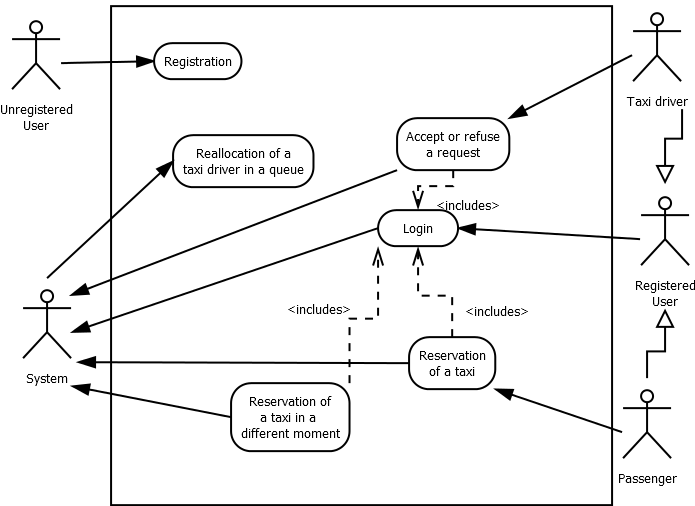
\includegraphics[scale=0.5]{Use Case.png}
\end{figure}

\pagebreak
\subsection{Non Functional Requirements}
\subsubsection{Performance Requirements}
The overall performance of the system must be acceptable so that a good level of usability is achieved.
The response time with the respect to the system must be near to zero. The response time of mobile application is tricky to evaluate since there are lots of different devices with different power processing, but  in general the application should perform well on the majority of the devices available in today market. Some very low level or entry level devices might show some delays rendering the application on the screen. Nevertheless the major bound is customers and drivers internet connection. 
\subsubsection{Design Constraints}
\subsubsection{Software System Attributes}
\paragraph{Availability} The overall system must be available anytime according to \hyperref[a10]{[A10]}. Dedicated servers must be used to reach this goal. In order to achieve even more reliability, some fault tolerant mechanisms must be implemented, also to reduce risks of high loads that could eventually result in denials of service. Servers must be replicated to work in parallel by multiple instances of the same application. 
\paragraph{Maintainability} The application provides specific APIs that will be documented, as the whole application.
\paragraph{Portability} The mobile application will be developed on all the major mobile OSes available in the market, also web application is portable since nowadays the majority of widespread OSes have a browser. The web application will be designed with a responsive layout to be also accessible from mobile devices as well. The business logic in the servers will be implemented using the Java language.
\subsubsection{Security}
\paragraph{External Interface Side}
\paragraph{Application Side}
\paragraph{Server Side}
\end{document}
